\chapter{Deep}\label{chap: deep}

Since this task considers only scores above the threshold,~\cite{boyd2012accuracy} named it \AccatTop. The important distinction from standard classifiers is that this threshold is no longer fixed, as in the case of~$0.5$, but depends on all samples. Therefore, the objective is non-additive and non-decomposable. This brings both theoretical and numerical issues. Standard machine learning algorithms use minibatch sampling. However, when the threshold is computed on a minibatch, it provides a lower estimate of the true threshold. Therefore, the sampled threshold is a biased estimate of the true threshold. Figure~\ref{fig:thresholds1} illustrates this phenomenon. The bias between the true and sampled thresholds is large even for medium-sized minibatches. Backpropagation then propagates this sampling error through the whole gradient, and consequently, the minibatch gradient is a biased estimate of the true gradient. This brings numerical issues~\cite{bottou2018optimization}.

\begin{figure}[!ht]
  \centering
  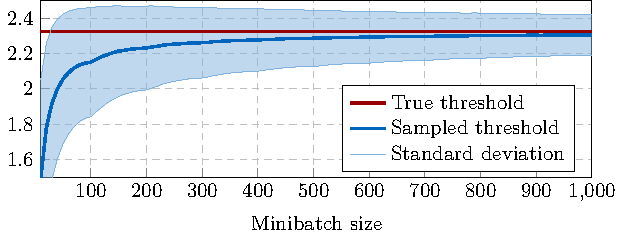
\includegraphics[width = \linewidth]{images/deep_threshold_bias.pdf}
  \caption{The bias between the sampled and true thresholds computed from scores following the standard normal distribution. The threshold separates the top~$1\%$ of samples with the highest scores.}
  \label{fig:thresholds1}
\end{figure}

\begin{figure*}[!ht]
  \centering
  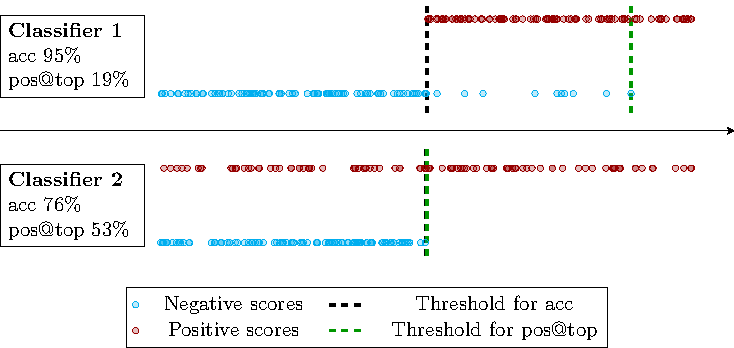
\includegraphics[width = \linewidth]{images/standard_aatp_comparison.pdf}
  \caption{Difference between standard classifiers (top row) and classifiers maximizing accuracy at the top (bottom row). While the former has a good total accuracy, the latter has a good top acccuracy.}
  \label{fig:difference}
\end{figure*}

Our method mitigates this bias. It is based on several results.~\cite{li2014top} proposed the TopPush formulation of the accuracy at the top and solved it in its dual formulation.~\cite{adam2021general} solved the TopPush formulation directly in its primal form for linear classifiers. Since we generalize the linear TopPush into non-linear classifiers, we name our method \DeepTopPush. We stay in the primal form to be able to employ stochastic gradient descent. Due to non-decomposability, we need to propose a way of computing the gradient and reduce the bias mentioned above. Since the threshold always equals to one of the scores~\cite{boyd2012accuracy}, its computation has a simple local formula. We implicitly remove some variables and apply the chain rule (backpropagation) to compute the gradient in an end-to-end manner. To reduce the bias, we need to improve the approximation quality of the sampled threshold. We employ again the fact that the true threshold corresponds to one sample. Since this sample changes slowly during optimization, we modify the idea of~\cite{adam2019machine} and enhance the current minibatch by the sample, which equalled the sampled threshold on the previous minibatch. As this added sample usually propagates across multiple minibatches, it tracks the threshold, and this trick mitigates the sampled threshold bias. The main contributions of the paper are as follows:
\begin{itemize}
  \item We propose \DeepTopPush, which is a simple and scalable method for accuracy at the top.
  \item We show that \DeepTopPush increases the computational time only slightly, yet it achieves better performance than prior art methods.
  \item We show both theoretically and numerically that enhancing the minibatch by one sample reduces the bias of the sampled gradient.
\end{itemize}
The paper is organized as follows: Section~\ref{sec:deeptheory} introduces a general formulation of accuracy at the top. Section~\ref{sec:solving} derives formulas for the bias of the sampled threshold and proposes \DeepTopPush to minimize it. Section~\ref{sec:numerics} shows the good performance of \DeepTopPush on multiple images recognition datasets, a real-world medical application, and a malware detection dataset, where we detected 46\% malware at an extremely low false alarm rate of~$10^{-5}$. To promote reproducibility, our codes are available online.

\section{Accuracy at the top}\label{sec:deeptheory}

This section introduces the accuracy at the top. A standard deep network~$f$ with weights~$\bm{w}$ takes inputs~$\bm{x}_i$, transforms them into scores~$z_i$, and computes the total loss based on these scores and labels~$y_i$. On the other hand, accuracy at the top solves
\begin{equation}\label{eq:problem}
  \begin{aligned}
    \minimize{w,z,t}
    & \lambda_1 \sum_{i\in I^-}\II_{z_i \ge t} + \lambda_2\sum_{i\in I^+}\II_{z_i < t} \\
    \st
    & z_i = f(\bm{w};\bm{x}_i), \\
    & t = G(\{(z_i, y_i)\}_{i\in I}).
  \end{aligned}
\end{equation}
Similarly to the standard network, the classifier~$f$ computes the score~$z_i$ for each sample~$\bm{x}_i$. Then a general function~$G$ takes the scores and labels of \textbf{all} samples and computes the threshold~$t$. This makes the problem non-decomposable. The objective function equals the weighted sum of false-positives (negative samples above the threshold) and false-negatives (positive samples below the threshold). Here,~$I$,~$I^+$ and~$I^-$ are the sets of all, positive and negative labels, respectively, and~$\II$ is the characteristic ($0/1$) function counting how many times the argument is satisfied. Setting \eqref{eq:problem} includes TopPush~\cite{li2014top} which minimizes the number of positive samples below the highest-ranked negative sample. This fits into \eqref{eq:problem} with~$\lambda_1=0$,~$\lambda_2=1$ and~$t=\max_{i\in I^-} z_i$.

Figure~\ref{fig:difference} shows the difference between the standard approach with cross-entropy and accuracy at the top. While classifier 1 has good total accuracy, its top accuracy is subpar because of the few negative outliers. On the other hand, classifier 2 has worse total accuracy, but its top accuracy is extremely good because more than half of the positive samples are on the top. While classifier 1 selected different thresholds for the accuracy and top metrics, these thresholds coincide for classifier 2.

Table~\ref{table:summary} shows other special cases of \eqref{eq:problem} including maximizing precision at a given level of recall~\cite{mackey2018constrained} or recall at~$K$. The threshold~$t$ always equals to the sample with the~$j^*$-th highest score on all, positive, or negative samples. The problems differ only in~$j^*$ and from which samples the threshold is computed. For example, Pat\&Mat-NP~\cite{adam2021general} minimizes the false negative rate (equivalently maximizes the true positive rate) under the constraint that the false positive rate is at most~$\tau$.

\begin{table}[!ht]
  \centering
  \begin{tabular}{@{}llllll@{}}
    \toprule
    Name &~$\lambda_1$ &~$\lambda_2$ & $t$ computed from & $j^*$ \\
    \midrule
    Prec@Rec    & $1$ & $0$ & positive samples & $\npos\tau$ \\
    Rec@K       & $0$ & $1$ & all samples      & $K$ \\
    TopPush     & $0$ & $1$ & negative samples & $1$ \\
    Pat\&Mat-NP & $0$ & $1$ & negative samples & $\nneg\tau$ \\
    \bottomrule
  \end{tabular}
  \caption{Selected problems of setting \eqref{eq:problem}. False-positives and false-negatives have weights~$\lambda_1$ and~$\lambda_2$, the threshold~$t$ equals to the sample with the~$j^*$-th highest score on all, positive, or negative samples.}
  \label{table:summary}
\end{table}

\subsection{Related works}

There is a close connection between accuracy at the top and ranking problems~\cite{batmaz2019review,werner2019review}. This was, together with similarities to the Neyman-Pearson problem, showed in~\cite{adam2021general}. A special case of the ranking problems attempts to rank positive samples above negative samples. Several approaches, such as RankBoost~\cite{freund2003efficient}, Infinite Push~\cite{agarwal2011infinite} or~$p$-norm push~\cite{rudin2009pnorm} employ a positive-negative pairwise comparison of scores, which can handle only small datasets. TopPush~\cite{li2014top} converts the pairwise sum into a single sum and minimizes the false-negatives below a threshold given by the maximum score corresponding to negative samples. Thus, it converts ranking into accuracy at the top problems.

Two approaches for solving \eqref{eq:problem} exist. The first approach considers the threshold constraint as it is, while the second approach uses heuristics to approximate it. In the first approach, Acc@Top~\cite{boyd2012accuracy} argues that the threshold equals one of the scores. They fix the index of a sample and solve as many optimization problems as there are samples.~\cite{eban2017scalable,adam2021general,kumar2021implicit} write the threshold as a constraint and replace both the objective and the constraint via surrogates.~\cite{eban2017scalable} uses Lagrange multipliers to obtain a minimax problem,~\cite{mackey2018constrained} implicitly removes the threshold as an optimization variable and uses the chain rule to compute the gradient while~\cite{macha2020nonlinear} solves an SVM-like dual formulation with kernels.~\cite{grill2016learning} uses the same formulation but applies surrogates only to the objective and recomputes the threshold after each gradient step. TFCO~\cite{cotter2019optimization} solves a general class of constrained problems via a minimax reformulation. In the second approach, SoDeep~\cite{engilberge2019sodeep} or SmoothI~\cite{thonet2021smoothi} use the fact that the threshold may be easily computed from sorted scores. They approximate the sorting operator by a network trained on artificial data. AP-Perf~\cite{fathony2019ap} considers a general metric and hedges against the worst-case perturbation of scores. The authors argue that the problem is bilinear in scores and use duality arguments. However, the bilinearity is lost when optimizing with respect to the weights of the original network. 

\section{DeepTopPush as a method for maximizing accuracy at the top}\label{sec:solving}

This section first shows a basic algorithm to solve \eqref{eq:problem}. We then argue that the stochastic gradient descent produces a biased estimate of the true gradient, and we mention two strategies for mitigating this bias. Based on one strategy, we propose the \DeepTopPush algorithm. The whole section assumes that the classifier~$f$ is differentiable.

\subsection{Basic algorithm for solving accuracy at the top}

Even though the presented technique can be applied to any formulation from Table~\ref{table:summary}, for simplicity, we derive it only for the TopPush formulation, where~$\lambda_1=0$ and~$\lambda_2=1$. This amounts to minimizing the false-negatives in \eqref{eq:problem}. Since the function~$\II$ in the formulation \eqref{eq:problem} is discontinuous, it is usually replaced by a general surrogate function~$l$ which is continuous and non-decreasing. This leads to
\begin{equation}\label{eq:problem_surr1}
  \begin{aligned}
    \minimize{w,z,t}
    & \frac{1}{\npos}\sum_{i\in I^+}l(t-z_i) \\
    \st
    & z_i = f(\bm{w};\bm{x}_i), \\
    & t   = G(\{(z_i, y_i)\}_{i\in I}).
\end{aligned}
\end{equation}
To apply the stochastic gradient descent, we need to compute the gradient. The core idea follows~\cite{mackey2018constrained} which was proposed in a more general context in~\cite{adam2019machine}. It rewrites problem \eqref{eq:problem_surr1} into its equivalent form
\begin{equation}\label{eq:problem_surr2}
  \minimize{w}
  \frac{1}{\npos}\sum_{i\in I^+}l\Brac{G\Brac{\{(f(\bm{w};\bm{x}_j), y_j)\}_{j\in I}} - f(\bm{w};\bm{x}_i)}.
\end{equation}
This form removed the constraints and it has the advantage that the only optimization variable is~$\bm{w}$ instead of~$(\bm{w}, \bm{z}, t)$ in \eqref{eq:problem_surr1}. In all cases from Table~\ref{table:summary}, the threshold~$t$ always equals to one of the scores, let it have index~$j^*$ and then~$t=z_{j^*}$. Denoting the objective of \eqref{eq:problem_surr2} by~$L(\bm{w})$, the chain rule implies that the gradient of the objective from \eqref{eq:problem_surr2} equals to
\begin{equation}\label{eq:grad1}
  \nabla L(\bm{w}) = \frac{1}{\npos} \sum_{i\in I^+}l'(t-z_i)\big(\nabla_w f(\bm{w};\bm{x}_{j^*}) - \nabla_w f(\bm{w};\bm{x}_i)\big).
\end{equation}
The stochastic gradient descent replaces the sum over all positive samples~$I^+$ with a sum over all positive samples in a minibatch~$\Imin^+$. However, as both the threshold~$t$ and the index~$j^*$ depend on all scores~$z_i$, they need to be approximated on the minibatch as well. We denote these approximations by~$\hat t$ and~$\hat j$, respectively. Denoting the number of positive samples in the minibatch by~$\nmin^+$, we replace the true gradient \eqref{eq:grad1} by the \textit{sampled gradient}
\begin{equation}\label{eq:grad2}
  \nabla \hat L = \frac{1}{\nmin^+}\sum_{i\in \Imin^+}l'(\hat t-z_i)\big(\nabla_w f(\bm{w};\bm{x}_{\hat j}) - \nabla_w f(\bm{w};\bm{x}_i) \big),
\end{equation}
The most straightforward way is to choose the sampled threshold~$\hat t$ by the same rule as the true threshold~$t$. As an example, if~$t$ is the~$100^{\rm th}$ largest score on the whole dataset and~$\frac{n}{\nmin}=20$ is the ratio of sizes of the whole dataset and of the minibatch, we select the sampled threshold~$\hat t$ as the~$5^{\rm th}$ largest score on the minibatch. We summarize this procedure in Algorithm~\ref{alg1}.

\begin{figure*}
  \begin{minipage}{0.48\textwidth}
    \begin{algorithm}[H]
      \centering
      \begin{algorithmic}[1]
        \State Initialize weights~$\bm{w}$
        \Repeat
        \State Select minibatch~$\Imin$
        \State \phantom{$\Iminh$}
        \State Compute~$z_i\gets f(\bm{w};\bm{x}_i)$ for~$i\in\Imin$
        \State Set~$\hat t \gets G(\{(z_i,y_i)\}_{i\in\Imin})$
        \State 
        \State Compute~$\nabla \hat L$ based on~$\Imin$\phantom{$\Iminh$}
        \State Make a gradient step
        \Until{stopping criterion is satisfied}
      \end{algorithmic}
      \caption{Basic algorithm for solving \eqref{eq:problem} \\}
      \label{alg1}
    \end{algorithm}
  \end{minipage}
  \hfill
  \begin{minipage}{0.48\textwidth}
    \begin{algorithm}[H]
      \centering
      \begin{algorithmic}[1]
        \State Initialize weights~$\bm{w}$, random index~$j^*$
        \Repeat
        \State Select minibatch~$\Imin$
        \State Enhance minibatch~$\Iminh = \Imin \cup \{j^*\}$
        \State Compute~$z_i\gets f(\bm{w};\bm{x}_i)$ for~$i\in\Iminh$
        \State Set~$\hat t \gets \{\max z_i \mid i\in \Iminh \cap I^-\}$
        \State Find index~$j^*$ such that~$t = z_{j^*}$
        \State Compute~$\nabla \hat L$ based on~$\Iminh\cap I^+$
        \State Make a gradient step
        \Until{stopping criterion is satisfied}
      \end{algorithmic}
      \caption{DeepTopPush as an efficient method for maximizing accuracy at the top.}
      \label{alg2}
    \end{algorithm}
  \end{minipage}
\end{figure*}

\subsection{Bias of the sampled gradient}

Convergence proofs of the stochastic gradient descent require that the sampled gradient is an unbiased estimate of the true gradient~\cite{bottou2018optimization}. This means that
\begin{equation}\label{eq:defin_bias}
  \bias(\bm{w}) := \nabla L(\bm{w}) - \EE \nabla \hat L(\bm{w})
\end{equation}
equals to~$0$ for all~$\bm{w}$. A comparison of \eqref{eq:grad1} and \eqref{eq:grad2} shows that a necessary condition is that the sampled threshold~$\hat t$ is an unbiased estimate of the true threshold~$t$. However, the sampled version underestimates the true value, which is evident for the maximum where the sampled maximum is always smaller or equal to the true maximum. The next result quantifies the difference between the sampled and true thresholds.

\begin{proposition}[\cite{glynn1996importance}]\label{proposition:bound}
  Let~$X$ be an absolutely continuous random variable with distribution function~$F$, let~$X_1,\dots,X_n$ be iid samples from~$X$ and let~$\tau\in(0,1)$. Denote the true threshold~$t=F^{-1}(1-\tau)$ and the sampled threshold~$\hat t=X_{[\lceil n\tau\rceil]}$. If~$F$ is differentiable with a positive gradient at~$t$, then
  \begin{equation*}
    \sqrt{n}(t - \hat t) \rightarrow N\left(0, \frac{\tau(1-\tau)}{F'(t)^2}\right),
  \end{equation*}
  where the convergence is in distribution and~$N$ denotes the normal distribution.
\end{proposition}

This proposition states that when the minibatch size increases to infinity, the variance of the sampled threshold is approximately~$\frac{\tau(1-\tau)}{nF'(t)^2}$. Figure~\ref{fig:thresholds1} in the introduction shows this empirically for the case where the scores follow the standard normal distribution and~$\tau=0.01$ is the desired top fraction. The approximation is poor with both large bias and standard deviation. Even though this result gives us insight into the bias of the sampled threshold, we are ultimately interested in the bias of the sampled gradient~$\nabla \hat L(\bm{w})$. To do so, recall that~$j^*$ is the threshold index on the whole dataset ($t=z_{j^*}$) while~$\hat j$ is the threshold index on the minibatch ($\hat t=z_{\hat j}$). We split the computation based on whether these two indices are identical.

\begin{lemma}\label{lemma:convergence}
  Let~$j^*$ be unique. Assume that the selection of positive and negative samples into the minibatch is independent and that the threshold is computed from negative samples while the objective is computed from positive samples. Then the conditional expectation of the sampled gradient satisfies
  \begin{equation*}
    \EE\Brac{\nabla \hat L(\bm{w}) \mid \hat j=j^*} =  \nabla L(\bm{w}).
  \end{equation*}
\end{lemma}
\begin{proof}
  If~$j^*$ is unique, then the true threshold~$t$ is a differentiable function. The differentiability of~$L$ and~$\hat L$ follows from the chain rule. If~$\hat j=j^*$ holds, then the sampled gradient equals to
  \begin{equation}\label{eq:grad_min_aux}
    \nabla \hat L(\bm{w})= \frac{1}{\nmin^+}\sum_{i\in \Imin^+}l'(t-z_i)\big(\nabla_w f(\bm{w};\bm{x}_{j^*}) - \nabla_w f(\bm{w};\bm{x}_i) \big).
  \end{equation}
  The summands are identical to the ones in \eqref{eq:grad1}. Since the sum is performed with respect to positive samples, the threshold is computed from negative samples, the lemma statement follows.
\end{proof}

Now we present the main result about the bias.

\begin{theorem}\label{theorem:convergence}
  Under the assumptions of Lemma~\ref{lemma:convergence}, the bias of the sampled gradient from \eqref{eq:defin_bias} satisfies
  \begin{equation}\label{eq:comp_bias}
    \bias(\bm{w}) = \PP(\hat j\neq j^*) \Brac{\nabla L(\bm{w}) - \EE\Brac{\nabla \hat L(\bm{w}) \mid \hat j\neq j^*}}.
  \end{equation}
\end{theorem}
\begin{proof}
  The law of total expectation implies
  \begin{equation*}
    \begin{aligned}
      \EE \nabla \hat L(\bm{w})
      & = \PP(\hat j=j^*)\EE(\nabla \hat L(\bm{w}) \mid \hat j=j^*) \\
      & \qquad + \PP(\hat j\neq j^*)\EE(\nabla \hat L(\bm{w}) \mid \hat j\neq j^*),
    \end{aligned}
  \end{equation*}
  from where the statement follows due to definiton \eqref{eq:defin_bias} and Lemma~\ref{lemma:convergence}.
\end{proof}

The assumptions of Theorem~\ref{theorem:convergence} holds for all methods from Table~\ref{table:summary} with the exception of Rec@K. For this method, the bias contains an additional term, as we show in the appendix.

The bias \eqref{eq:comp_bias} consists of a multiplication of two terms. We propose two strategies for reducing the bias. The first strategy reduces both terms, while the second strategy reduces only the first term.

\subsection{Bias reduction: Increasing minibatches size}\label{sec:bias1}

The natural choice to mitigate the bias is to work with large minibatches. Even though this is not a standard way, some works suggest this route~\cite{you2019large}. When the minibatch is large, it contains more samples and the chance that~$\hat j$ differs from~$j^*$ decreases. This reduces the first term in~\eqref{eq:comp_bias}. Moreover, Proposition~\ref{proposition:bound} ensures that the difference between the sampled threshold~$\hat t$ and the true threshold~$t$ is small. Then the difference between the true gradient \eqref{eq:grad1} and the sampled gradient \eqref{eq:grad2} decreases as well. This reduces the second term in \eqref{eq:comp_bias}. This approach is applicable to any method from Table~\ref{table:summary}.

\subsection{Bias reduction: Incorporating delayed values}\label{sec:bias2}

Various reasons may enforce the use of small minibatches. Then Algorithm~\ref{alg1} is not suitable for a small fraction of top samples. For example, a minibatch of size~$32$ with~$16$ negative samples must have thresholds~$\tau\ge \frac{100}{16}=6.25\%$. However, we need to aim for much smaller thresholds.

We propose a simple fix based on the reasoning that when the weights~$\bm{w}$ of a neural network are updated, the scores~$\bm{z}$ usually do not change much, especially for a small learning rate. This means that if a sample has the largest score, it will likely have the largest score even after the gradient step. Since the threshold~$t$ for TopPush equals the largest score corresponding to negative samples, we can easily track it. We enhance the current minibatch by the negative sample from the previous minibatch with the highest score. This significantly increases the chance that the sampled threshold is the true threshold and, due to the first term in \eqref{eq:comp_bias}, reduces the bias of the sampled gradient.

We summarize the procedure in Algorithm~\ref{alg2} and show it next to Algorithm~\ref{alg1} to highlight the differences. In every iteration, it stores the index~$j^*$ of the sample, which equals the threshold (step~7). We add it to the enhanced minibatch (step 4). Since we can track only the maximum, we set the threshold as the maximum of scores from negative samples (step~6) and minimize false-positives. Since Algorithm~\ref{alg2} uses the same formulation as \textit{TopPush}~\cite{li2014top} but can handle an arbitrary classifier, we name it \DeepTopPush. We provide empirical evidence of why our technique works later in Section~\ref{sec:delay}.
